\section{Benutzerumfrage über die Feuerwehr-Community}

Ein wichtiger Aspekt der Silvanet-Anwendung ist die Benachrichtigung und Anzeige von Informationen über das Entstehen eines Waldbrandes und dessen Verfolgung in Echtzeit.
Es ist jedoch zu beachten, dass die Anwendung nicht für den Gebrauch durch Feuerwehrleute bestimmt ist.
Eine von Dryad im Vorfeld durchgeführte interne Untersuchung zeigte, dass die große Mehrheit der Feuerwehrleute seit vielen Jahren mit bestimmten Computer- oder anderen Lösungen arbeitet.
Der Versuch, mit dieser Gewohnheit durch eine noch so gut genutzte Anwendung zu konkurrieren, wäre also ein Misserfolg.

Die Anwendung beschränkt sich also darauf, die Informationen an den für den Standort verantwortlichen Kunden weiterzuleiten, der dann selbst die örtlichen Behörden und die Feuerwehr kontaktieren muss, die dann wie bisher die Arbeit übernehmen wird.
Die Feuerwehrleute, die auf den Platz gehen, sind nämlich nicht die Feuerwehrleute, die bei einem Notfall mit der Nummer 911 z. B. gerufen werden.
Diejenigen, die angerufen werden und die Informationen über den Notfall erhalten, heißen \textit{Dispatchers}.
Sie entscheiden anhand der erhaltenen Informationen, wie viele Einheiten wohin geschickt werden und leiten die Informationen an die Feuerwehrleute weiter, die vor Ort sind.
Eine Situation, in der ein Waldbrand entdeckt wird, kann also mit dem folgenden Use-Case-Diagramm schematisiert werden:

\begin{figure}[H]
  \centering
  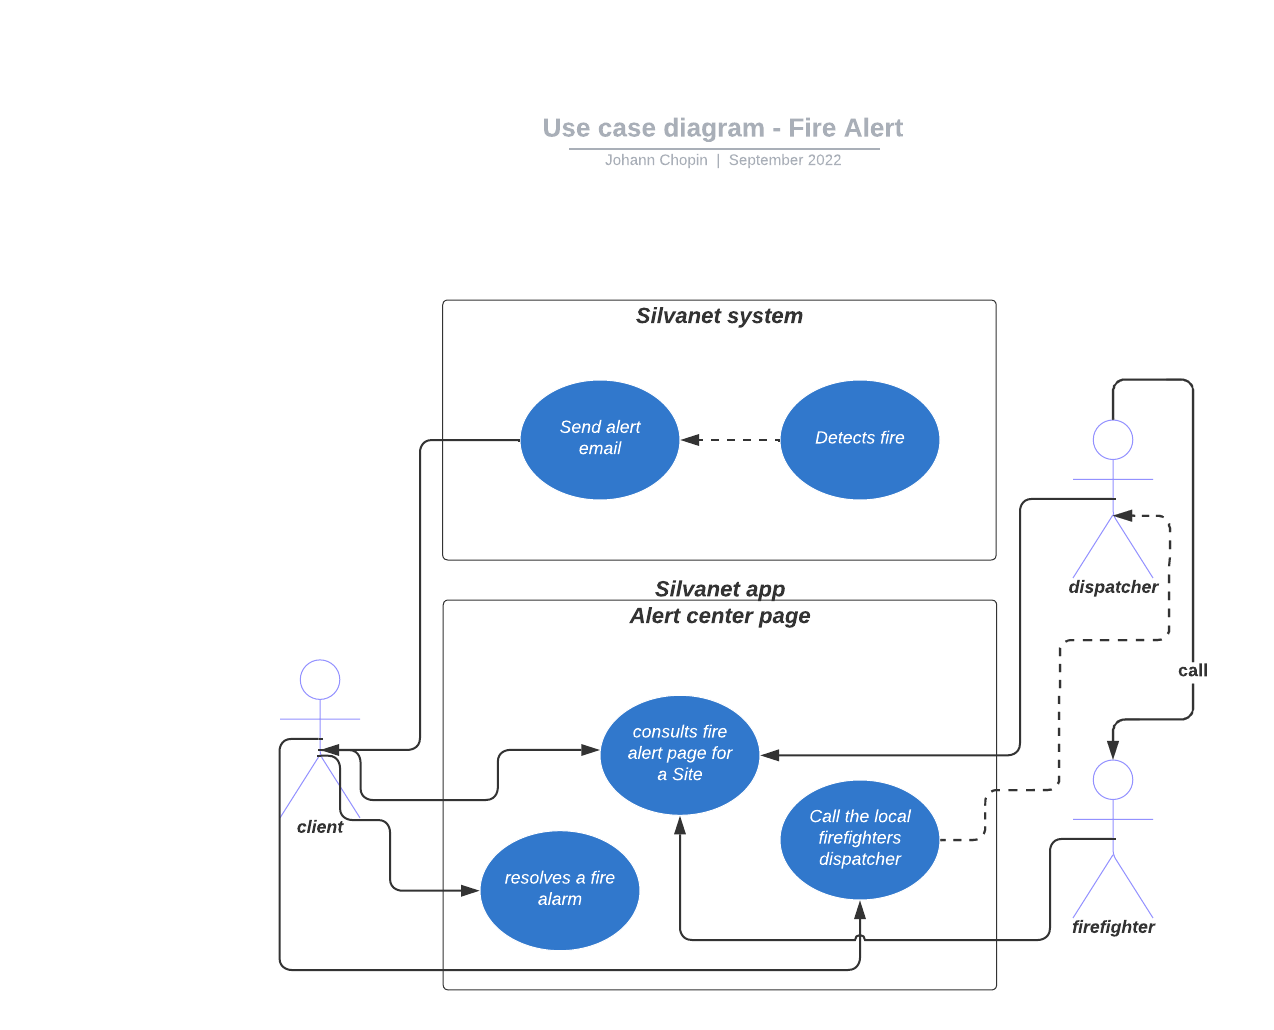
\includegraphics[width=\textwidth]{use_case_diagram_dispatcher}
  \caption{Use-case-diagram, das Kunden, Dispatchers, Feuerwehrleute, das Silvanet-System (Netzwerk von Sensoren im Wald) und die Silvanet-Anwendung bei der Erkennung eines Waldbrandes verbindet.}
  \label{fig:use_case_diagram_dispatcher}
\end{figure}

Mit dieser Darstellung kann man sehen, dass, auch wenn die Anwendung nicht direkt von Feuerwehrleuten genutzt wird (obwohl es für sie möglich ist, sie zu konsultieren), es notwendig ist, dass die Schnittstelle dem Benutzer relevante Informationen anzeigt, sodass er sie kurz und bündig und schnell an die Dispatchers weitergeben kann.
Daher ist es notwendig, genauer zu wissen, was die Feuerwehrleute wissen müssen und wie sie in einer Notsituation wie einem Waldbrand vorgehen.
Da wir keine relevanten Ressourcen gefunden haben, die alle Fragen beantworten, die eine Verbesserung der Silvanet-Schnittstelle ermöglichen, ist eine interne Suche erforderlich.

\subsection{Definition des Fragebogenumfangs}

Wie bei allen Benutzertests ist es notwendig, vorab festzulegen, was das Ziel der Untersuchung ist und wie es erreicht werden soll.
In diesem Sinne war es auch notwendig, dass Entscheidungen von der Gruppe und nicht von Einzelpersonen getroffen wurden, um so viele Ideen wie möglich abzudecken.
Außerdem war noch nicht klar, welches Medium für die Untersuchung verwendet werden sollte, und es gab viele Möglichkeiten, Informationen zu sammeln, z. B. Interviews, Fragebögen oder A/B-Vergleichstests.
Ein von \citeauthor{customerQuestionBoard} entwickeltes Framework für UX-Forschung namens \citetitle{customerQuestionBoard} ermöglicht es, das Problem mit Hilfe von Brainstorming-Sitzungen im Team zu entwirren und ein geeignetes Medium für die Forschung zu definieren.
Diese Methode ist in 7 Schritte unterteilt:

\begin{enumerate}
  \item \textbf{Vorbereitung}: Der erste Schritt besteht darin, sicherzustellen, dass das Team das Ziel der Forschung versteht und weiß, welche Art von Rückmeldungen sie liefern soll.
  \item \textbf{Eingabeaufforderung}: Bitten Sie das Team, Fragen auf Klebezettel zu schreiben, einen Klebezettel pro Frage. Die Frage sollte auf die Frage "Was wollen wir über Feuerwehrleute lernen?
  \item \textbf{Diskutieren und Clustern}: Bitten Sie jeden Benutzer einzeln, seine Klebezettel nach passenden Kategorien zu gruppieren. Die Idee ist zu sehen, wie Fragen auf viele verschiedene Arten gestellt werden können.
  \item \textbf{Einstellung und Verhalten}: Fragen Sie das Team für jedes Cluster, ob sich die Frage auf die Einstellung oder das Verhalten des Kunden bezieht who \textit{Einstellung} ist das, was Menschen über ein Produkt oder eine Dienstleistung sagen oder denken und \textit{Verhalten} ist das, was Menschen mit dem Produkt oder tun ist. Stellen Sie Einstellungsfragen auf der linken Seite und Verhaltensfragen auf der rechten Seite.
  \item \textbf{Qualitativ und quantitativ}: Fragen Sie das Team, ob es bei den Fragenbündeln darum geht, herauszufinden, warum etwas passiert und wie man es beheben kann (qualitative Fragen). Oder darum, wie oft oder wie viel etwas passiert (quantitative Fragen). Danach stellen Sie quantitative Fragen auf der rechten Seite und qualitative Fragen auf der linken Seite.
  \item \textbf{Priorität festlegen}: Im vorherigen Punkt wurden die Fragecluster in vier Gruppen eingeteilt. Das Team muss nun festlegen, welche Gruppe am relevantesten ist.
  \item \textbf{Fragen zu Methoden und Hilfsmitteln zuordnen}: Für das Cluster, das die meisten Stimmen erhalten hat, kann das Team nun herausfinden, welche Nutzerforschungsmethode es anwenden soll. Das Cluster oben rechts verwendet qualitative und strukturierte Methoden. Das Cluster oben links verwendet qualitative und unstrukturierte Methoden. Der untere linke Quadrant verwendet qualitative und indirekte Methoden. Der untere rechte Quadrant verwendet quantitative und indirekte Methoden.
\end{enumerate}

Die Aktivierung wurde vom Dryad Cloud-Team mit dem Miro-Tool durchgeführt. Das Ergebnis ist das folgende Clustering. Die einzelnen Schritte des Prozesses können im Anhang \ref{appendix:question_board} nachgelesen werden.

\begin{figure}[H]
  \centering
  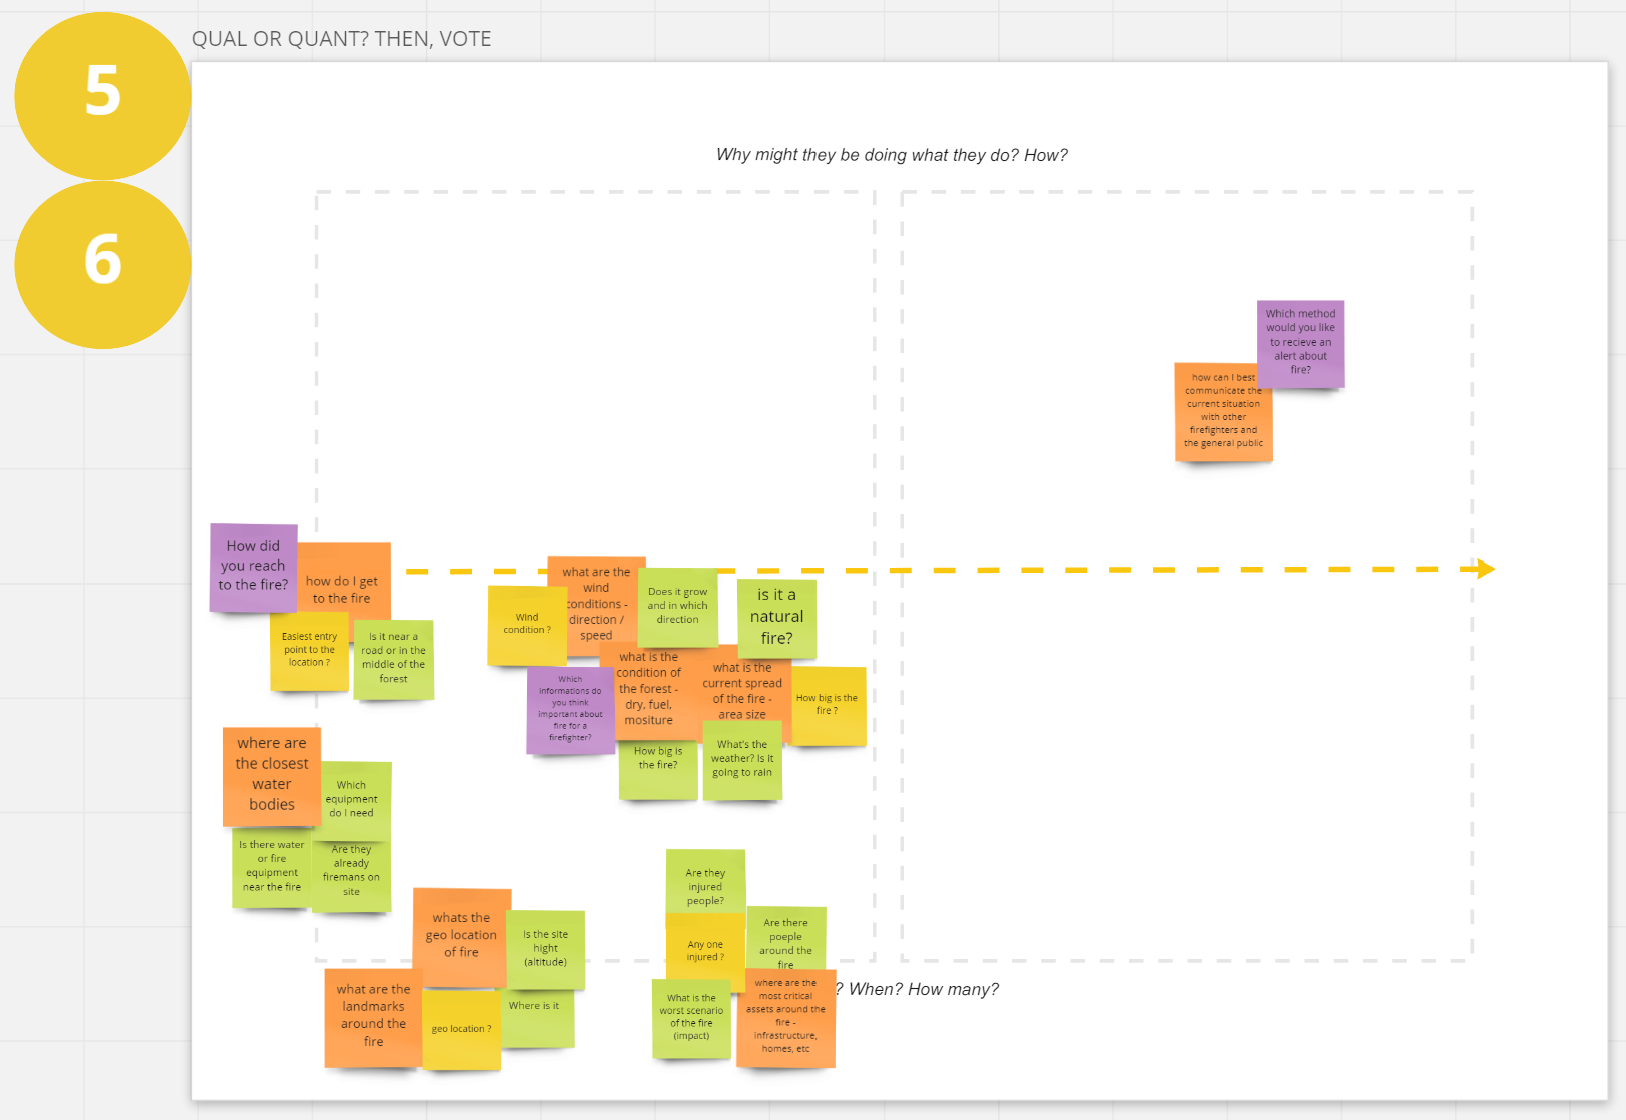
\includegraphics[width=\textwidth]{question_board_5}
  \caption{Ergebnis der UX-Methode des Question Board}
  \label{fig:question_board_5_not_appendix}
\end{figure}
